\documentclass[border=6pt]{standalone}
\usepackage[T1]{fontenc}
\usepackage{lmodern}
\usepackage{amssymb}
\usepackage{array}
\usepackage{tikz}
\usetikzlibrary{arrows.meta,calc}
\usepackage{pgfplots}
\pgfplotsset{compat=1.18}
\definecolor{cardblue}{HTML}{114d95}
\definecolor{oldorange}{HTML}{7d1f1b}
\definecolor{aqua}{HTML}{deb520}
\definecolor{notsure}{HTML}{A8A69E}
\newcommand{\pieslice}[4]{%
  \fill[#3, draw=white, line width=1.2pt] (0,0) -- (#1:\R) arc[start angle=#1, end angle=#2, radius=\R] -- cycle;
  \node[font=\small\bfseries, text=white] at ({(#1+#2)/2}:{0.62*\R}) {#4};}
\begin{document}
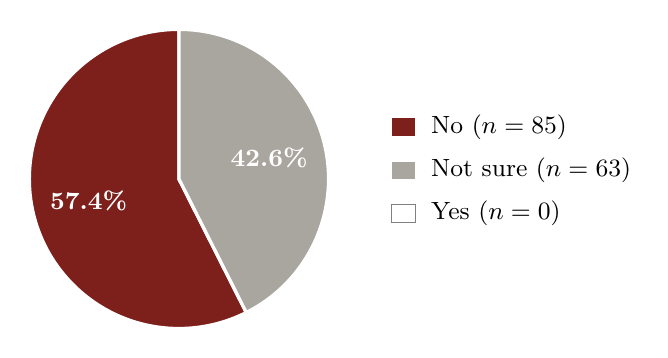
\begin{tikzpicture}
  \def\R{1.9}
  \pieslice{90}{296.76}{oldorange}{57.4\%}
  \pieslice{296.76}{450}{notsure}{42.6\%}
  \begin{scope}[xshift=2.7cm, yshift=0.55cm, font=\small]
    \fill[oldorange] (0,0) rectangle (0.3,0.22);       \node[anchor=west] at (0.38,0.11) {No ($n=85$)};
    \fill[notsure]   (0,-0.55) rectangle (0.3,-0.33);  \node[anchor=west] at (0.38,-0.44) {Not sure ($n=63$)};
    \draw[black!50]  (0,-1.10) rectangle (0.3,-0.88);  \node[anchor=west] at (0.38,-0.99) {Yes ($n=0$)};
  \end{scope}
\end{tikzpicture}
\end{document}
